\lab{Method of Mean Weighted Residuals}{Method of Mean Weighted Residuals}
\label{lab:pseudospectral1_revision}
\objective{We introduce the method of mean weighted residuals (MWR) and use it to derive a pseudospectral method. This method will then be used to solve several boundary value problems.}

Consider a linear differential equation 
\[Lu = f, \]
defined on the interval $[-1,1]$, together with associated boundary conditions. 
We will approximate the solution $u(x)$ by a linear combination of $N+1$ basis functions $\phi_i$, so that 
\[
u(x) \approx u_N(x) = \sum_{i=0}^N a_i \phi_i(x). 
\]
To determine appropriate constants $a_i$, we then minimize the residual function 
\[
R(x,u_N) = Lu_N - f.
\]
Note that $R(x,u) = Lu - f = 0$ for the true solution $u(x)$.

This general strategy is often called the method of mean weighted residuals (MWR method). The MWR method is a general framework that describes many other, more specific methods. These more specific methods come from differing approaches to minimizing the residual $R(x,u_N)$, and the choice of basis functions $\phi_i$.


\section*{The Pseudospectral Method}
The pseudospectral or collocation method is obtained from the MWR method by forcing the residual function $R(x,u_N)$ to equal zero at $N+1$ points in $[-1,1]$, called collocation points. 
When done correctly, the pseudospectral method gives high accuracy and converges rapidly. 

We will let the basis functions $\phi_i$ be the Chebychev polynomials, and the collocation points will be the Gauss-Lobatto points, $x_i = \cos(\pi i /N)$, $ i = 0, \ldots, N$.
The appropriate solution $u_N$ may be represented with two equivalent forms. 
First, $u_N$ can be described with the first $N+1$ coefficients  $\{a_i\}_{i=0}^N$ of its expansion in the Chebychev polynomials. 
Since $u_N$ is a polynomial of order $N$, it may be uniquely described by its values at the collocation points, that is, the unknown values  $\{u_N(x_i)\}_{i=0}^N$.

These equivalent forms satisfy
\begin{align}
	MA = F \label{spectral1b:chebychev_expansion}
\end{align}
and
\begin{align}
	LU &= F \label{spectral1b:grid_point}
\end{align}
where 
\begin{align*}
	U_i &= u(x_i),\\
	A_i &= a_i,\\
	F_i &= f(x_i),\\
	L_{ij} &= \left.(LC_j(x))\right|_{x=x_i},\\
	M_{ij} &= \left.(L\phi_j(x))\right|_{x=x_i}. 
\end{align*}

The functions $C_j$ above are the cardinal functions, defined to be the polynomials of least degree satisfying
\begin{equation*}
C_j(x_i) = \begin{cases} 1 & i=j \\ 0 & i \not = j.
   \end{cases}
\end{equation*}
Thus, $u_N$ can also be expanded in the basis of the cardinal functions: 
\begin{align*}
	u_N(x) &= \sum_{j=0}^N u_N(x_j)C_j(x).
\end{align*}

When $L = d/dx$, the matrix corresponding to equation \eqref{spectral1b:grid_point} is given by 
\begin{align*}
L_{ij} &= \frac{dC_j}{dx}(x_i) = 
\begin{cases} (1+2N^2)/6 & i=j=0, \\ -(1+2N^2)/6 & i=j=N, \\
-x_j/[2(1-x_j^2)] & i=j, \, 0<j<N, \\ 
(-1)^{i+j}\alpha_i/[\alpha_j(x_i-x_j)] & i \not = j.
   \end{cases}
\end{align*}
where $\alpha_0 = \alpha_N = 2,$ and $\alpha_j = 1$ otherwise. 

This matrix is often called the differentiation matrix ($D$), and can be used to piece together the matrix $L$ for more complicated differential operators. 
A stable, vectorized function to build the differentiation matrix is given below. 


\begin{lstlisting}
import numpy as np

def cheb(N):
	x =  np.cos((np.pi/N)*np.linspace(0,N,N+1))
	x.shape = (N+1,1)
	lin = np.linspace(0,N,N+1)
	lin.shape = (N+1,1)
	
	c = np.ones((N+1,1))
	c[0], c[-1] = 2., 2.
	c = c*(-1.)**lin
	X = x*np.ones(N+1) # broadcast along 2nd dimension (columns)
	
	dX = X - X.T
	
	D = (c*(1./c).T)/(dX + np.eye(N+1))
	D  = D - np.diag(np.sum(D.T,axis=0))
	x.shape = (N+1,)
	# Here we return the differentation matrix and the Chebychev points, 
	# numbered from x_0 = 1 to x_N = -1
	return D, x

\end{lstlisting}



\section*{Using the Differentiation Matrix}


\begin{problem}
Use the differentiation matrix to numerically approximate the derivative of $u(x) = e^{x}\cos(6x)$ on a grid of $N$ Chebychev points where $N=6, 8,$ and $10.$  
(Use the linear system $D U \approx U'$.)
Then use barycentric interpolation to approximate $u'$ on a grid of 100 evenly spaced points.

Graphically compare your approximation to the exact derivative. 
Note that this convergence would not be occurring if the collocation points were equally spaced. 
\end{problem}

To approximate $u''(x)$ on the grid $\{x_i\}$, we use 
\[U'' \approx D^2 U.\]
The BVP
\begin{align*}
&{ }u'' = f(x), \quad x \in [-1,1],\\
&{ }u(-1) = 0, \quad u(1) = 0,
\end{align*}
can be discretized by the linear system 
\begin{align}
	D^2 U &= F, \label{spectral1b:discretization}
\end{align}
where $F = [f(x_0),\ldots, f(x_N)]^T$.
Since we have Dirichlet boundary conditions of $0$, we can satisfy the boundary condition by forcing $U[0] = U[N] = 0$. 
This is done by replacing the first and last equations in \eqref{spectral1b:discretization} by the boundary conditions. 
% This allows us to ignore the first and last equations in the system, giving us the new system 
% \[\tilde{D}^2 \tilde{U} = \tilde{F},\]
% where $\tilde{D} = D[1:N,1:N]$, $\tilde{U} = U[1:N]$, and $\tilde{F} = F[1:N]$.


\begin{problem}
Use the pseudospectral method to solve the boundary value problem 
\begin{align*}
&{ } u'' = e^{2x}, \quad x \in [-1,1], \\
&{ } u(-1) = 0, \quad u(1) = 0.
\end{align*}
Compare your numerical solution with the exact solution, 
\[
u(x) = \frac{- \cosh(2) - \sinh(2)x + e^{2x}}{4}.
\]
\end{problem}

% \begin{figure}
% \centering
% 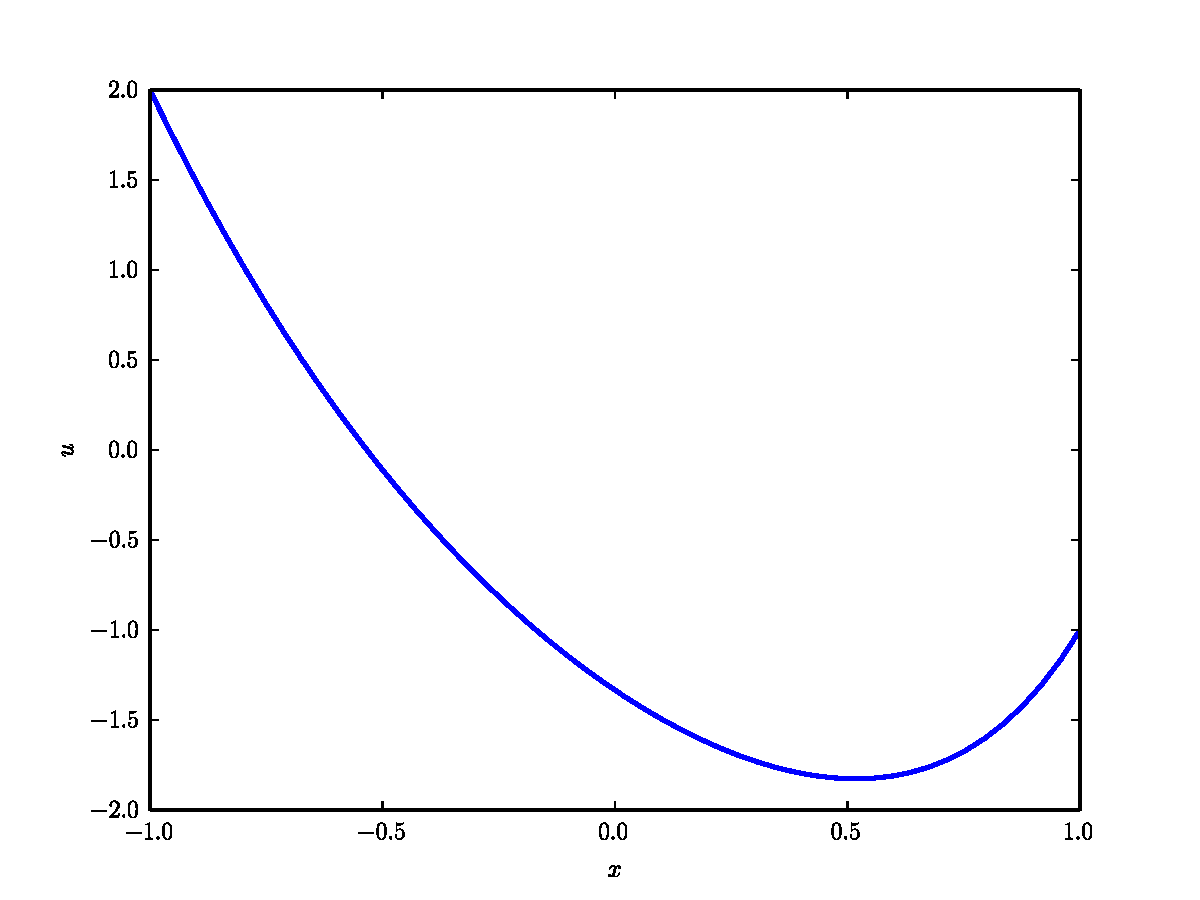
\includegraphics[width=\textwidth]{nonzeroDirichlet.pdf}
% \caption{The solution of $u'' + u' = e^{3x}$, subject to the boundary conditions 
% $u(-1) = 2$, $u(1) = -1$.}
% \label{fig:nonzeroDirichlet}
% \end{figure}

\begin{problem}
Use the pseudospectral method to solve the boundary value problem 
\begin{align*}
&{ } u'' + u' = e^{3x}, \quad x \in [-1,1], \\
&{ } u(-1) = 2, \quad u(1) = -1.
\end{align*}
% Check that your numerical solution is converging.
% How many subintervals are required to find the solution correct to three decimal places?
% See Figure \ref{fig:nonzeroDirichlet}.
	
% Hint: Reduce the problem to one with zero Dirichlet conditions by letting $u = U+G$, where $G$ is a (simple) function satisfying the boundary conditions.
\end{problem}





\section*{Minimizing the Area of a Surface of Revolution}
A surface of revolution that minimizes its area is an example of a larger class of surfaces called minimal surfaces. A famous example of a minimal surface is a soap bubble. Soap bubbles minimize their surface area while containing a fixed volume of air. This behavior extends to merged bubbles, and a soap film whose boundary is a wire frame. Minimal surfaces have applications in molecular engineering and material science, and general relativity, where they describe the apparent horizon of a black hole. 

Consider a function $y(x)$ defined on $[-1,1]$ satisfying $y(-1) = a $, $y(1) = b. $ The area of the surface obtained by revolving the graph of $y(x)$ about the $x$-axis is given by 
\[T[y(x)] = \int_{-1}^1 2 \pi y(x) \sqrt{1 + (y'(x))^2}\, dx .\]
To find the function $y(x)$ whose surface of revolution minimizes surface area, we must minimize the functional $T[y]$. 
This is a classical problem from a branch of mathematics called the calculus of variations. 
Standard derivatives allow us to find the minimum values of functions defined on $\mathbb{R}^n$, and where they occur. 
The calculus of variations allows us to find the minimum values of functions whose input are other functions. 

From the calculus of variations we know that a necessary condition for $y(x)$ to minimize $T[y]$ is that the Euler-Lagrange equation must be satisfied: 
\begin{align*}
	L_y - \frac{d}{dx}L_{y'} = 0,
\end{align*}
where $L(x,y,y') = 2 \pi y \sqrt{1 + (y')^2}$.  
Simplifying the Euler-Lagrange equation for our problem results in the ODE
\[y y'' - (y')^2 -1 = 0.\]
Discretizing this ODE using the pseudospectral method results in the (nonlinear) system of equations 
\[
Y \cdot (D^2 Y) - (DY) \cdot (DY) = I,
\]
where $I$ is a vector of ones.

\begin{problem}
Find the function $y(x)$ that satisfies $y(-1) = 1$, $y(1) = 7$, and whose surface of revolution (about the $x$-axis) minimizes surface area. 
Compute the surface area, and plot the surface. \label{prob:pseudospectral1_revision:minimal_surface}
\end{problem}

\begin{figure}
\centering
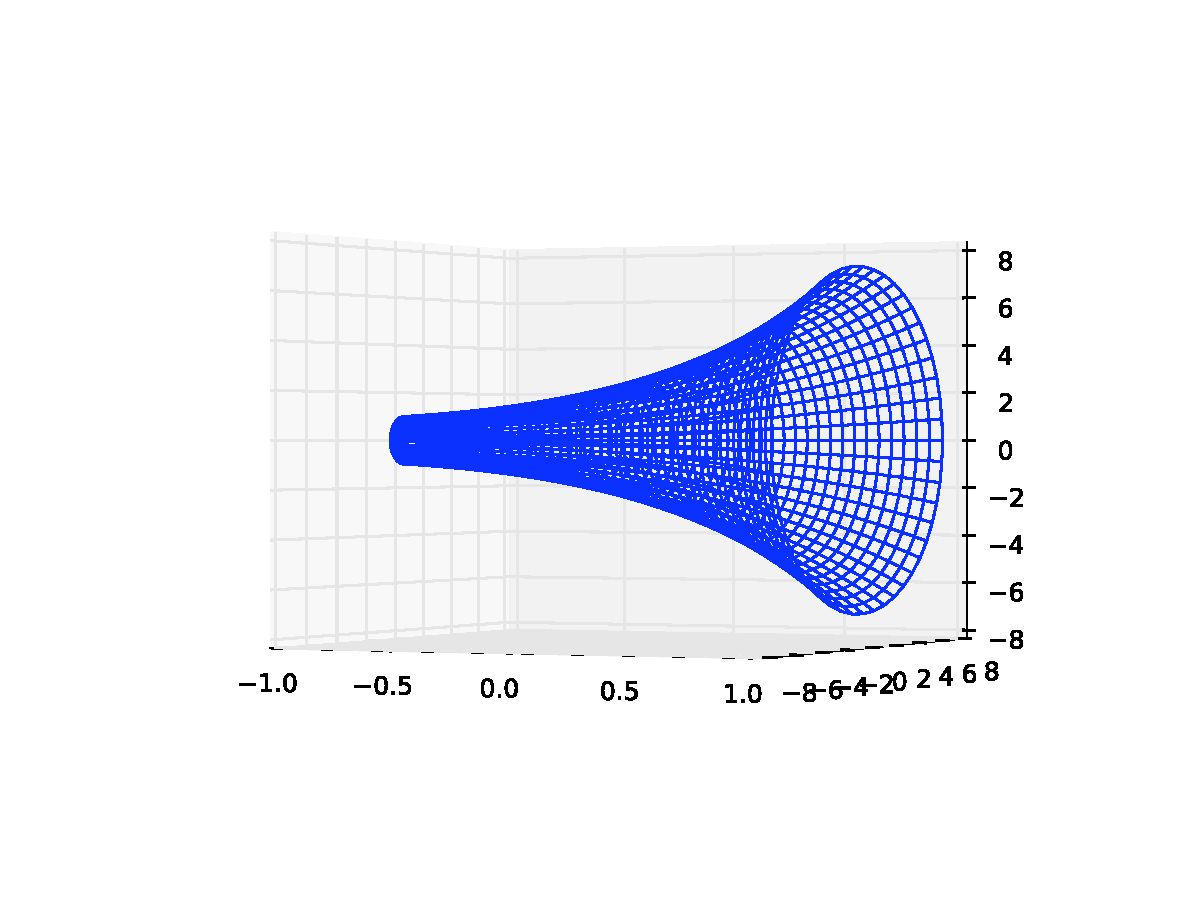
\includegraphics[width=\textwidth]{minimal_surface.pdf}
\caption{The minimal surface corresponding to Problem  \ref{prob:pseudospectral1_revision:minimal_surface}.}
\label{fig:pseudospectral1_revision:minimal_surface}
\end{figure}








\begin{comment}
\section*{The Method of Weighted Residuals}
We may write our differential/integral equation in operator notation as 
\[(Lu)(x) = f(x), \quad x \in \Omega\]
where $u$ belongs to some infinite-dimensional function space $V.$
We seek for an approximation $u_N$ to the solution $u$.
Our approximation $u_N$ will come from a finite-dimensional function space $S_N$ called the trial space.
Here we use $N$ to denote the dimension of $S_N \subset V$. 
The space $S_N$ can be described by a basis $\{\phi_1(x), \ldots, \phi_N(x)\}$.
Then an approximation $u_N \in S_N$ has the form 
\[u_N = \sum_{j=1}^N \gamma_j \phi_j\]

We can then define an operator $\mathcal{R}$ on the trial space $S_N$ by 
\[\mathcal{R}u_N(x) = Lu_N(x) - f(x)\] 
$\mathcal{R}u_N$ is called the residual or the error of the trial function $u_N$.
Note that the residual of the true solution $u$ is zero.
The method of weighted residuals is a family of methods that determine the coefficients $\gamma_j$ of the approximate solution $u_N$ by forcing the residual $\mathcal{R}u_N$ to be zero in some weighted average over $\Omega$.
In other words, given some collection of weight/test functions $\{w_i\}_{i=1}^M$, we require that 
\begin{align}
\int_{\Omega}\mathcal{R}u_N(x) w_i(x)\, dx &= 0, \quad \text{ for } i = 1, \ldots M
\label{eqn:Spectral1_weightedaverage}
\end{align}

After doing the integration described by (\ref{eqn:Spectral1_weightedaverage}), we obtain a system of algebraic equations that may be used to determine the coefficients $\gamma_i$.
Different choices of the trial space $S_N$ and the weight/test functions $w_i(x)$ result in different methods. 

We obtain the pseudospectral method (or collocation method) by choosing a collection of points $\{x_i\}_{i=1}^M$ in our space $\Omega$ called collocation points.
The weight functions $w_i(x)$ are then given by $w_i(x) = \delta(x-x_i); $ that is, $w_i$ is the Dirac delta function centered at $x_i$.
Then the equations \ref{eqn:Spectral1_weightedaverage} are given by 
\begin{align*}
	\int_{\Omega} \mathcal{R}u_N w_i(x) \, dx &= 0,\\
	\int_{\Omega} \mathcal{R}u_N \delta(x-x_i) \, dx &= 0, \\
	\mathcal{R}u_N(x_i) &= 0 \quad \text{ for } i = 1, \ldots, M
\end{align*}
Thus the pseudospectral method requires the residual of the approximate solution to be exactly zero at the collocation points.
Alternatively, the approximate solution satisfies the differential equation exactly at the collocation points. 
\end{comment}









